\documentclass[12pt, a4paper,oneside, openany]{book}
%fuente12pt,tamaño carta,una cara,quitar hojas en blanco,tipo libro
\usepackage[utf8]{inputenc} %fuente Unicode
%\usepackage[margin=-0cm]{geometry} %margen
\usepackage{graphicx} %uso de imagenes
\usepackage{multicol} %uso de multicolumnas
\usepackage{multirow} %multi celdas
\usepackage{lastpage} %n.total de paginas
\usepackage{colortbl} %columnas de color
\usepackage{tikz, tikz-3dplot} %figuras
\usepackage{tkz-euclide}
\usepackage{adjustbox} %manejo de margenes
\usepackage[spanish]{babel} %lenguaje español
\usepackage[document]{ragged2e} %alineacion
\usepackage[T1]{fontenc} %codificacion fuente
\usepackage{palatino} %fuente
\usepackage{enumerate} %viñeta numeros
\usepackage[colorlinks,linkcolor=myblue,citecolor=mygreen]{hyperref} %link personalizado
%-------------------------------------------------------------------
\definecolor{myblue}{HTML}{2D74B5} %color de titulos y subtitulos
%-------------------------------------------------------------------
\graphicspath{ {img/} } %localizacion de carpeta con imagenes
\renewcommand{\baselinestretch}{1.2} %espacio entre parrafos

%\AtBeginDocument{\AtBeginShipoutNext{\AtBeginShipoutDiscard}}
%elimina paginas adicionales que se agregan con el uso de hyperref

\usepackage{multirow} %multi celdas en tablas
\usepackage{longtable} %tablas multipagina
\usepackage{caption} %ajuste de tablas, figuras
\usepackage{color} %colores de texto
\usepackage{wrapfig} %rodear imagenes
\usepackage{booktabs, multirow} %bordes y rangos
\usepackage{titlesec} %titulos personalizados
\usepackage{eso-pic,picture} %imagenes con texto
\usepackage{nomencl} %simbolos de nomenclatura
\usepackage{lipsum} %crea texto default
\makenomenclature %tamaño nomenclatura
%\usepackage{showframe} %muestra el margen de las pg
%-------------------------------------------------------------------
%codigo del borde
\AddToShipoutPicture{%
\setlength\fboxsep{1pt}%
\put(24pt,24pt){\framebox(19.3066cm,28.0066cm)[lb]{}}%
}

%margenes
\usepackage{geometry}
\newgeometry{
        top=0.001in,
        bottom=3.2in,
        outer=0.55in,  %izquierda
        inner=0.55in, %derecha
        }
%-------------------------------------------------------------------
\usepackage{fancyhdr}%uso de encabezado y pie personalizado
\pagestyle{fancy}

\setlength{\headheight}{160pt}%ubicacion de caja de encabezado

\titlespacing{\chapter}{0pt}{-42pt}{0.5cm}%config capitulos, espacio de chapter
\titleformat{\chapter}[display]
{\sffamily\color{myblue}} {
  {\normalfont\color{myblue}\Large}
        \hspace{0pt}
            {\setlength\fboxsep{0pt}
                \colorbox{myblue}{
                }
            }
    }
  {0 pt}
  {\titlerule[0pt]\LARGE\sffamily}

%-------------------------------------------------------------------
\fancyhf{}%Declaración de encabezado
\pagestyle{fancy}
\fancypagestyle{plain}{}
%encabezado general
\begin{document}%inicio de documento
\lhead{

\begin{minipage}{0.1\textwidth}
\scalebox{1}[1.2]{
\begin{tabular}{|m{2cm}|m{10.8cm}|m{1.0cm}|m{1.0cm}|m{1.0cm}| }

\hline

\multirow{3}{2cm}{\centering
\includegraphics[width=1.0\textwidth]{tjacdmx_logo.png}}
& \footnotesize\centering\bf\sffamily{TRIBUNAL DE JUSTICIA ADMINISTRATIVA DE TABASCO}
& \footnotesize\bf\sffamily{Día}
& \footnotesize\bf\sffamily{Mes}
&\footnotesize\bf\sffamily{Año}
\\ \cline{2-5}

& \centering\bf\footnotesize\sffamily{DIRECCIÓN GENERAL DE ADMINISTRACIÓN}
& \footnotesize\centering\bf\sffamily{28}
& \footnotesize\centering\bf\sffamily{02}
& \footnotesize\bf\sffamily{2023}
\\ \cline{2-5}

& \centering\bf\footnotesize\sffamily{DIRECCIÓN DE INFORMÁTICA}
& \multicolumn{3}{ |c| }{\bf\footnotesize\sffamily{Versión: 001 }}
\\ \cline{2-5}

&
\centering\bf\footnotesize\sffamily{MANUAL DE USUARIO}
& \multicolumn{3}{ |c| } {\bf\footnotesize\sffamily{Página \thepage~de\ \pageref{LastPage}}}
\\ \hline

\end{tabular}}
\end{minipage}

}
%-------------------------------------------------------------------

\centerline{
\includegraphics[width=0.8\textwidth]{tjacdmx_logo.png}}%imagen de logo en portada
%titulo de portada

\vspace{1cm}%espacio
%-------------------------------------------------------------------
\begin{flushright}%alineación a la derecha

\newcommand{\ProjectTitle}

\vspace{0cm}
%titulo en portada
{\color{myblue}{\sffamily\large\bf\sffamily
ACTUARIA\\
ESTRADOS Y BOLETÍN ELECTRÓNICO\\
\vspace{0.3cm}
MANUAL DE USUARIO\\
\vspace{0.2cm}
DIRECCIÓN DE INFORMÁTICA}
}

\end{flushright}
%-------------------------------------------------------------------
%pie de todas las paginas
\cfoot[]{
{
\scalebox{1}[0.9]{%tamaño de celdas
\centering\begin{tabular}{|m{4cm}|m{4.0cm}|m{4.0cm}|m{4.0cm}| }

\hline

\centering\sffamily IDENTIFICACIÓN
& \centering\sffamily ELABORÓ
&  \centering\sffamily REVISÓ
& AUTORIZÓ
\\
\hline

\centering\sffamily TJACDMX DI MANUAL USUARIO
&  \centering\sffamily Dirección de Informática
&  \centering\sffamily Dirección de Informática
&  Pendiente de validación
\\
 \hline
\end{tabular}}

}}
%-------------------------------------------------------------------


\renewcommand{\headrulewidth}{0pt}%sin linea por default
\begin{quote}%alineacion de texto

\tableofcontents

\chapter{\large{Objetivo del sistema de información}}\label{chap:objetivo}
Con la finalidad de ofrecer a los servidores públicos del Tribunal de Justicia Administrativa de Tabasco
una herramienta que facilite la operación de los apartados que integran el módulo
de «Actuaría v 3.0», se elaboró el presente Manual.

\chapter{\large{¿Cómo ingresar a Actuaría v3.0?}}\label{chap:ingreso}

1.Ingresaremos al Sistema con el siguiente link:

\begin{center}
\href{https://sidj.tjacdmx.gob.mx}{https://sidj.tjacdmx.gob.mx}
\end{center}

2.Nos ubicaremos en el menú y daremos clic en  {\bf{
<<Actuaria v3.0>> }}

\begin{center}
    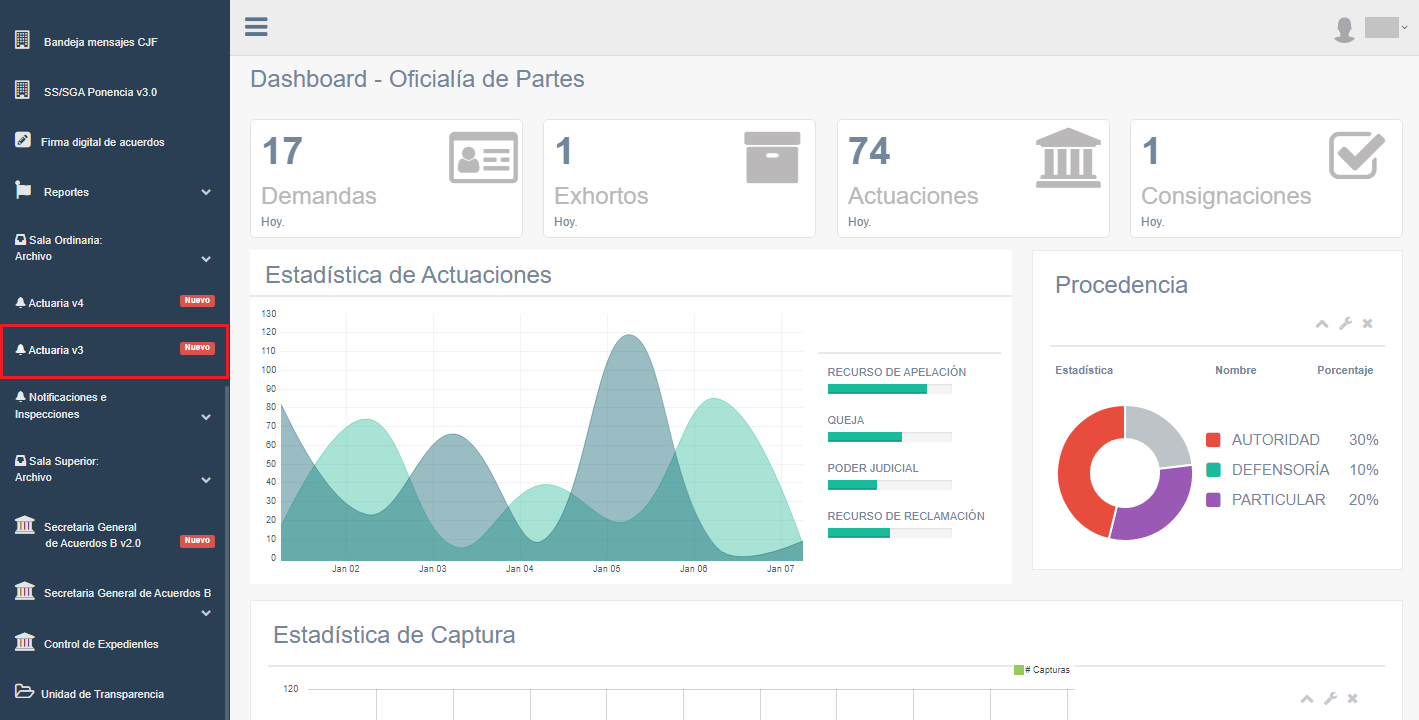
\includegraphics[width=0.88\columnwidth]{inicioAc.png}
\end{center}

\chapter{\large{Lista de estrados y boletín electrónico.}}\label{chap:boletin}

En el módulo de Listado de estrados y boletín electrónico podrá realizar las siguientes actividades:

\begin{itemize}
    \item Registro de listados.
    \item Escaneo de acuerdos.
    \item Consultar listados.
    \item Editar listados.
    \item Impresión de listados.
    \item Exportar listados.
\end{itemize}

{\bf{Datos del módulo consulta}}

\begin{enumerate}[(1)]
    \item Sección de búsqueda.
    \item Sección de listados de acuerdos
    \item Iconos 
\end{enumerate}
\begin{itemize}
    \item Imprimir
    \item Exportar
    \item Consultar
    \item Eliminar listado
\end{itemize}


\begin{center}
    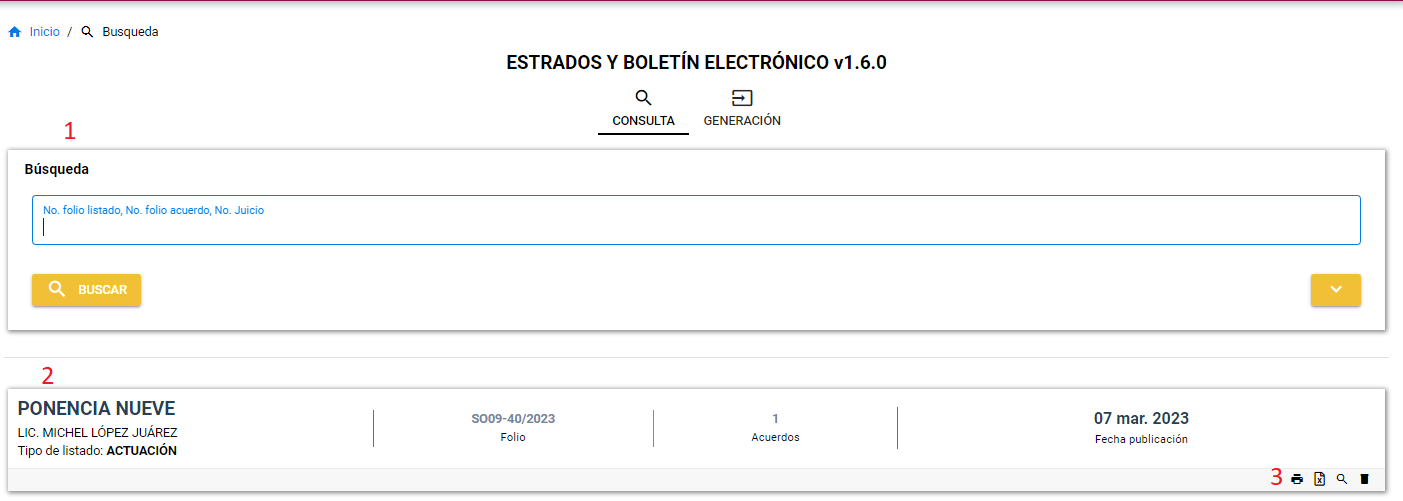
\includegraphics[width=0.88\columnwidth]{datos_consulta.png}
\end{center}


{\Huge{\color{myblue} \section{ ¿Cómo registrar un listado de acuerdos?}\label{sec:6}}}

\begin{center}
    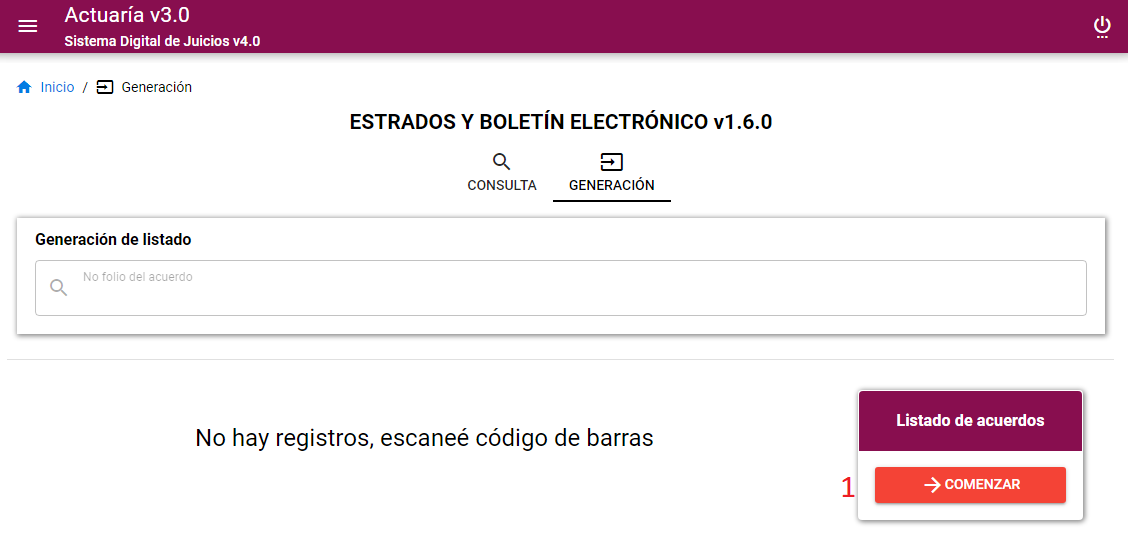
\includegraphics[width=0.88\columnwidth]{boletin.png}
\end{center}

1. Para generar un listado de acuerdos deberá dar clic en el botón {\bf «COMENZAR»} el cual presentará la
siguiente pantalla:

\begin{center}
    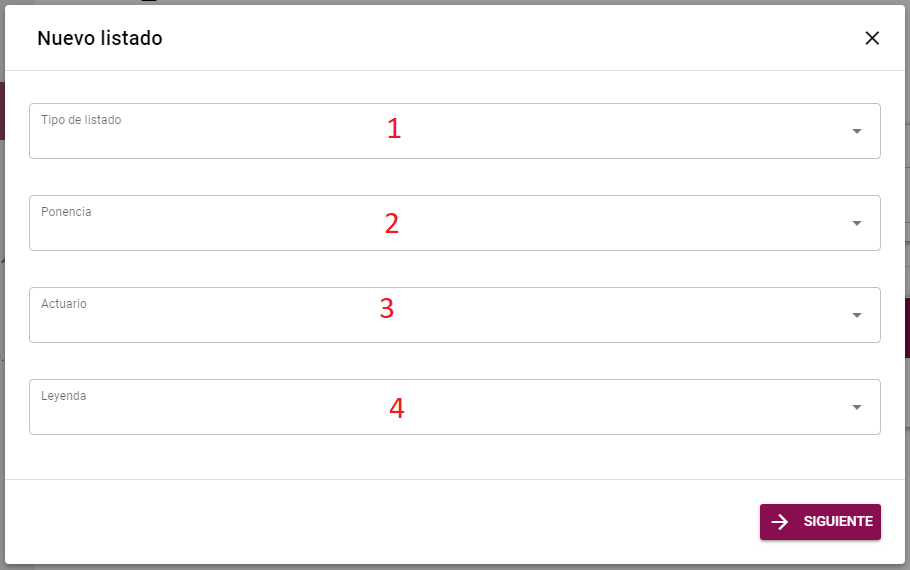
\includegraphics[width=0.66\columnwidth]{nuevo_list.png}
\end{center}

Tendrá que seleccionar las siguientes opciones:\\

\begin{enumerate}[1.]
    \item Tipo de listado
    \item Ponencia.
    \item Actuario
    \item Leyenda
\end{enumerate}

Después de llenar los 4 campos antes mencionados da clic en el botón {\bf «SIGUIENTE»} donde presentará la
siguiente pantalla:

\begin{center}
    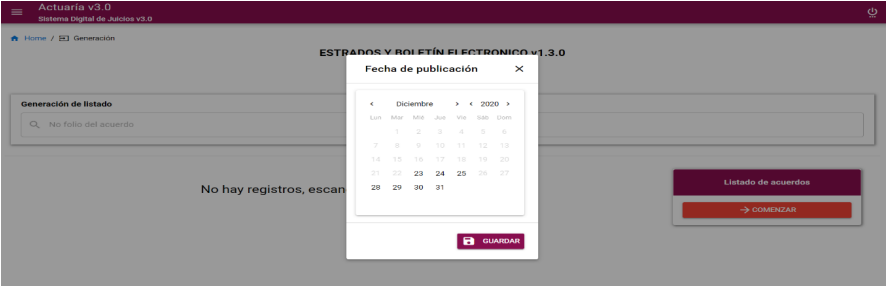
\includegraphics[width=0.88\columnwidth]{C16.png}
\end{center}

Seleccione la fecha de publicación de listado y da clic en el botón {\bf «GUARDAR»}, mostrará la siguiente
pantalla:

\begin{center}
    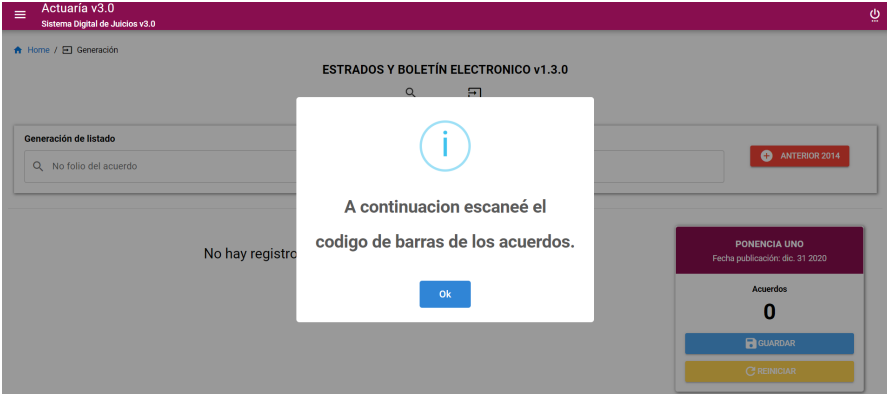
\includegraphics[width=0.88\columnwidth]{C17.png}
\end{center}

da clic en {\bf «OK»}, o espera 3 segundos y se quitara automáticamente.

{\Huge{\color{myblue} \section{ ¿Cómo escaneo el código de barras de los acuerdos?}\label{sec:7}}}

Para ingresar acuerdos en el listado, se podrá escanear el folio que se encuentra en la parte inferior del
acuerdo generado por el sistema digital de juicios.

\begin{center}
    
\includegraphics[width=0.30\columnwidth]{C18.png}
\end{center}

En el contenedor mostrará el listado de los acuerdos con la siguiente información:

\begin{itemize}
    \item Actor.
    \item Promoción.
    \item Número de juicio.
    \item Folio del acuerdo.
    \item Tipo de acuerdo.
\end{itemize}

\begin{center}
    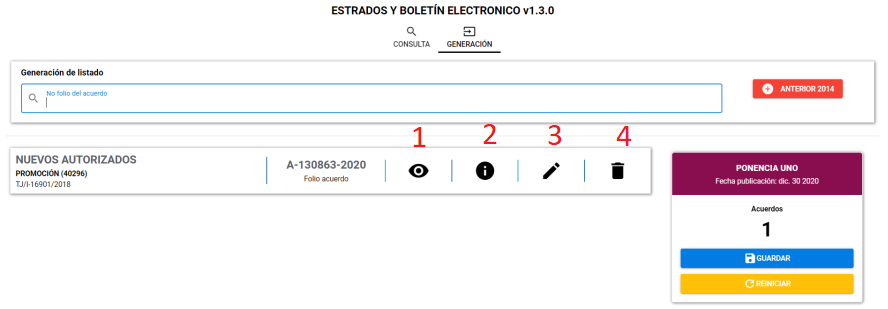
\includegraphics[width=0.88\columnwidth]{C19.png}
\end{center}

\begin{itemize}
    \item Podrá visualizar el acuerdo dando clic en el icono con el {\bf número {1}}.
    \item Podrá visualizar la información dando clic en el icono con el {\bf número {2}}
    \item Podrá editar la observaciones dando clic en el icono con el {\bf número {3}}.
    \item Podrá eliminar un acuerdo dando clic en el icono con el {\bf número {4}}.
    \item Podrá reiniciar el listado dando clic en el botón {\bf «REINICIAR»}.
\end{itemize}

Para terminar el registro de la lista deberá dar clic en el botón {\bf «GUARDAR»}, el sistema mostrara un mensaje de
confirmación y redireccionara al listado generado.

{\Huge{\color{myblue} \section{ ¿Cómo registrar juicios anteriores al año 2014?}\label{sec:8}}}

Para registrar juicios anteriores al 2014 solo deberá dar clic en el botón {\bf «ANTERIOR 2014»},

\begin{center}
    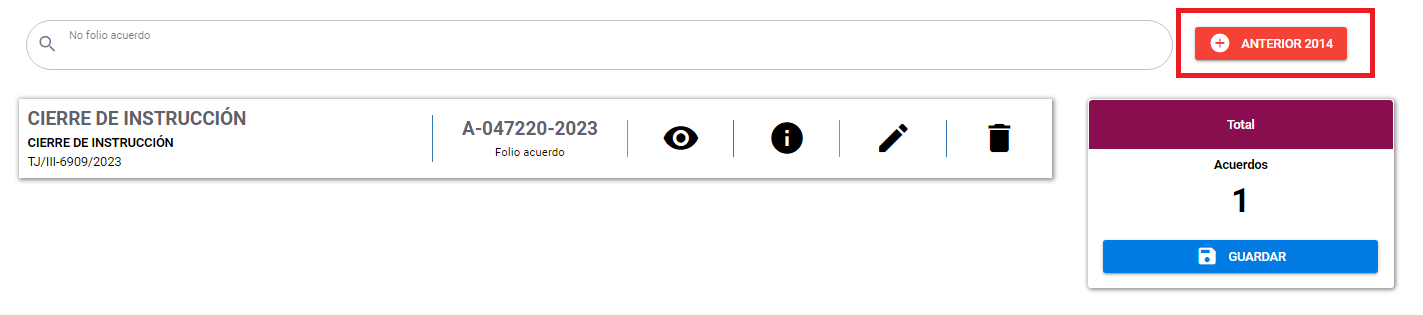
\includegraphics[width=0.88\columnwidth]{anterio2014.png}
\end{center}

Se mostrará la siguiente pantalla:

\begin{center}
    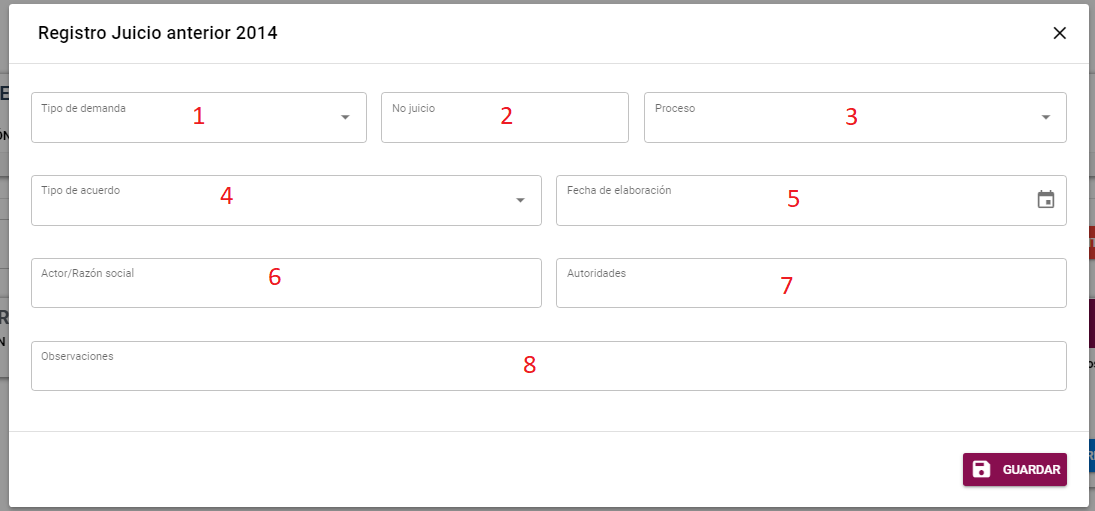
\includegraphics[width=0.88\columnwidth]{anterior2014.png}
\end{center}

Se requiere ingresar los siguientes datos ya que son campos obligatorios:

\begin{itemize}
    \item Tipo de demanda.
    \item Número de juicio.
    \item Proceso.
    \item Tipo de acuerdo.
    \item Fecha de elaboración.
    \item Actor/Razón social.
    \item Autoridades.
\end{itemize}

Las observaciones son opcionales, una vez que se ingresó toda la información, da clic en el botón
{\bf «GUARDAR»}, para que lo agregue a lista que ya se tiene generada.


{\Huge{\color{myblue} \section{ ¿Cómo buscar un listado de estrados?}\label{sec:9}}}

\begin{center}
    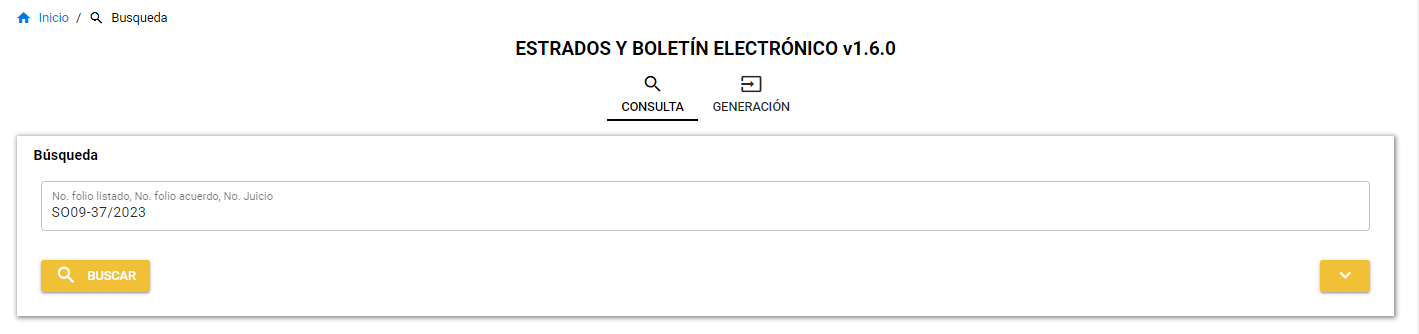
\includegraphics[width=0.88\columnwidth]{busqueda_bol.png}
\end{center}

Para poder realizar la búsqueda es necesario tener al menos uno de los siguientes datos que se
enlistan:

\begin{itemize}
    \item Número de listado.
    \item Número de folio del acuerdo.
\end{itemize}

Después de ingresar uno de los dos datos mencionados anteriormente debe dar clic el botón
{\bf «BUSCAR»}, para que muestre los resultados obtenidos.\\

Para obtener una búsqueda más avanzada y precisa de clic en el botón con el {\bf {número 1}} y se mostrará la siguiente pantalla.

\begin{center}
    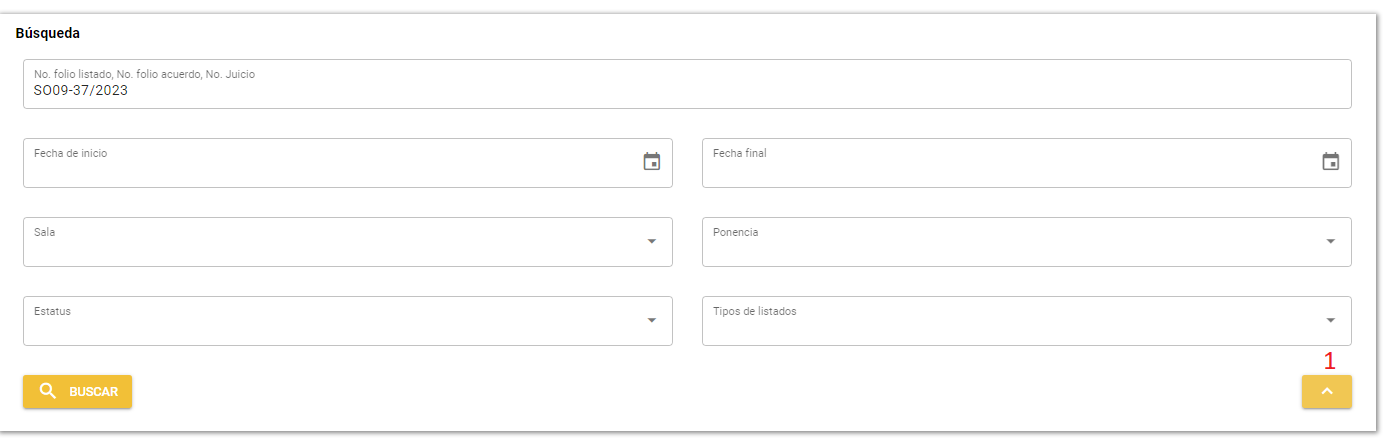
\includegraphics[width=0.88\columnwidth]{busqueda_avan.png}
\end{center}

La cual muestra los siguientes datos:

\begin{itemize}
    \item Número de listado, No. de folio acuerdo, No Juicio
    \item Fecha inicio.
    \item Fecha final.
    \item Sala.
    \item Ponencia.
    \item Estatus
    \item Tipo de listado
\end{itemize}

Ingresados los datos para la búsqueda solo debe de dar clic el botón de {\bf «BUSCAR»}, para que realice
la búsqueda y muestre los resultados obtenidos por el sistema.

{\Huge{\color{myblue} \section{ ¿Cómo editar un listado de estrados?}\label{sec:10}}}

Para poder editar un listado de estrados es necesario realizar la búsqueda de la lista como se describe anteriormente.

Una vez realizada la búsqueda mostrara la siguiente pantalla con los resultados obtenidos:

\begin{center}
    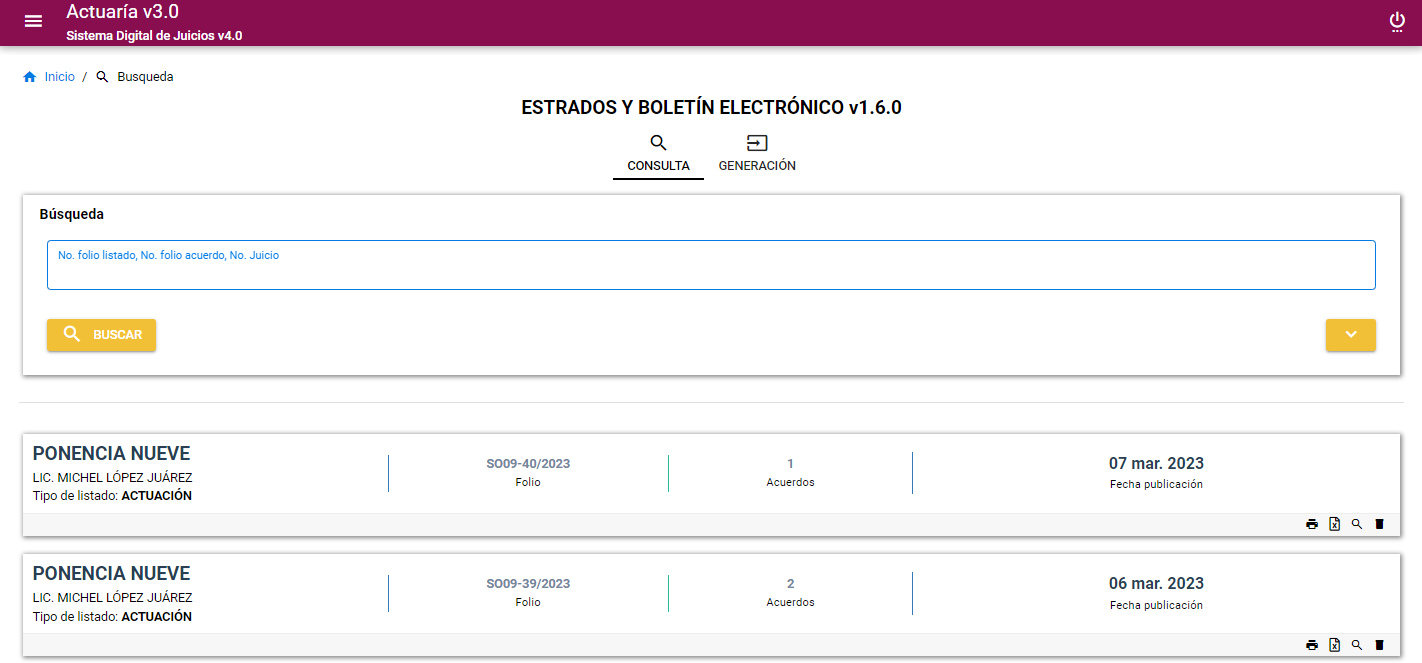
\includegraphics[width=0.88\columnwidth]{busqueda_list.png}
\end{center}

Da clic en icono de {\bf {<<Consultar>>}} que tiene forma de lupa.\\
Se mostrará una pantalla similar.

\begin{center}
    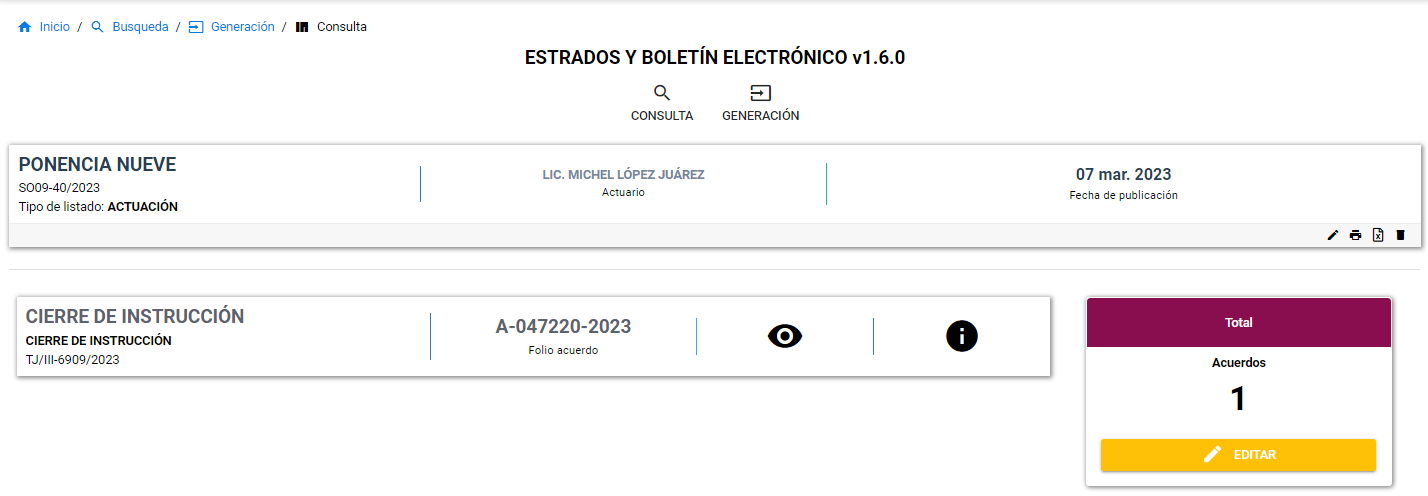
\includegraphics[width=0.88\columnwidth]{editar_list.png}
\end{center}

Ahí se presenta los datos del listado, con el número total de acuerdos que contiene la lista y los
datos de cada uno de los acuerdos. Para poder editar el listado deberá dar clic en el botón {\bf «EDITAR»},
para que presente las siguientes pantallas:

\begin{center}
    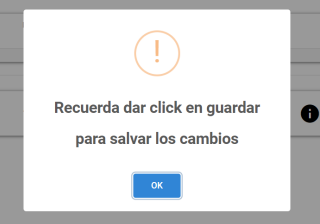
\includegraphics[width=0.44\columnwidth]{C27.png}
\end{center}

Muestra un mensaje de recordatorio para guardar los cambios realizados. Después presentara la siguiente pantalla:

\begin{center}
    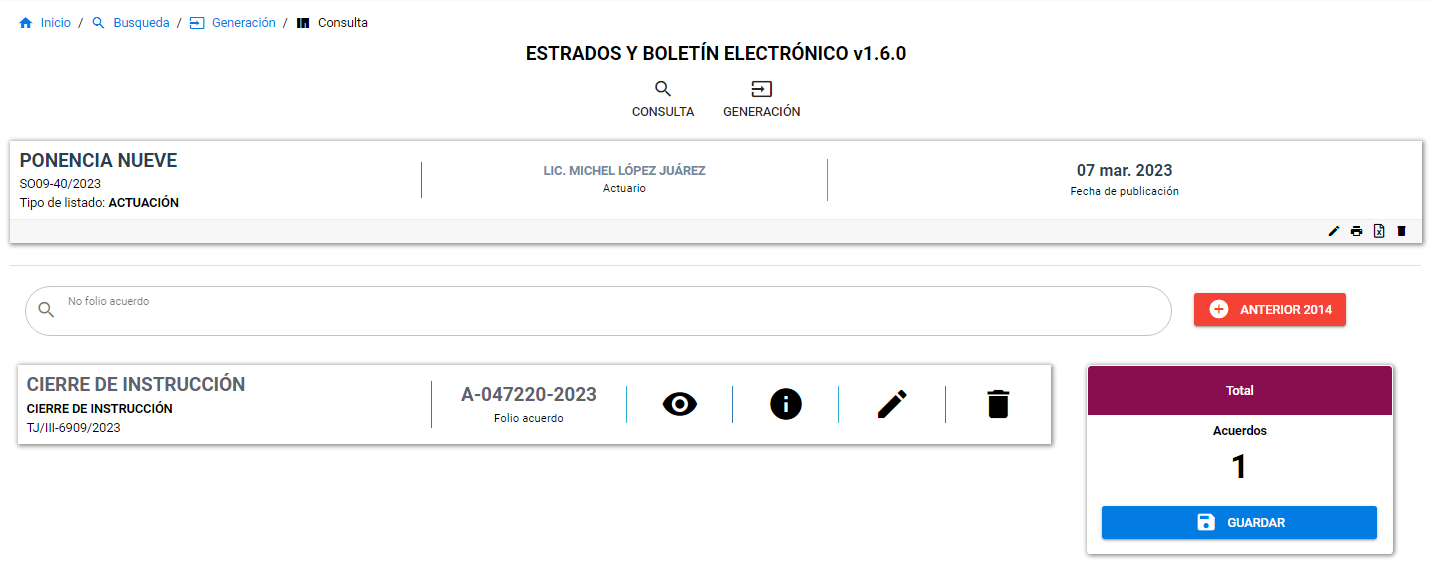
\includegraphics[width=0.88\columnwidth]{editar_list2.png}
\end{center}

Donde se ingresarán o escanearan los acuerdos
\textit{Ver ~\nameref{sec:6}}

{\bf NOTA: Recuerda dar clic el botón «GUARDAR», para que los cambios realizados se guarden.} 

{\Huge{\color{myblue} \section{ ¿Cómo se modifican los datos del listado (Ponencia, Actuario, Fecha de publicación y leyenda)?}\label{sec:11}}}

Para modificar la información del listado es necesario consultar el listado \textit{Ver ~\nameref{sec:9}} y dar clic en el icono {\bf{<<Editar>>}} como
se muestra a continuación:

\begin{center}
    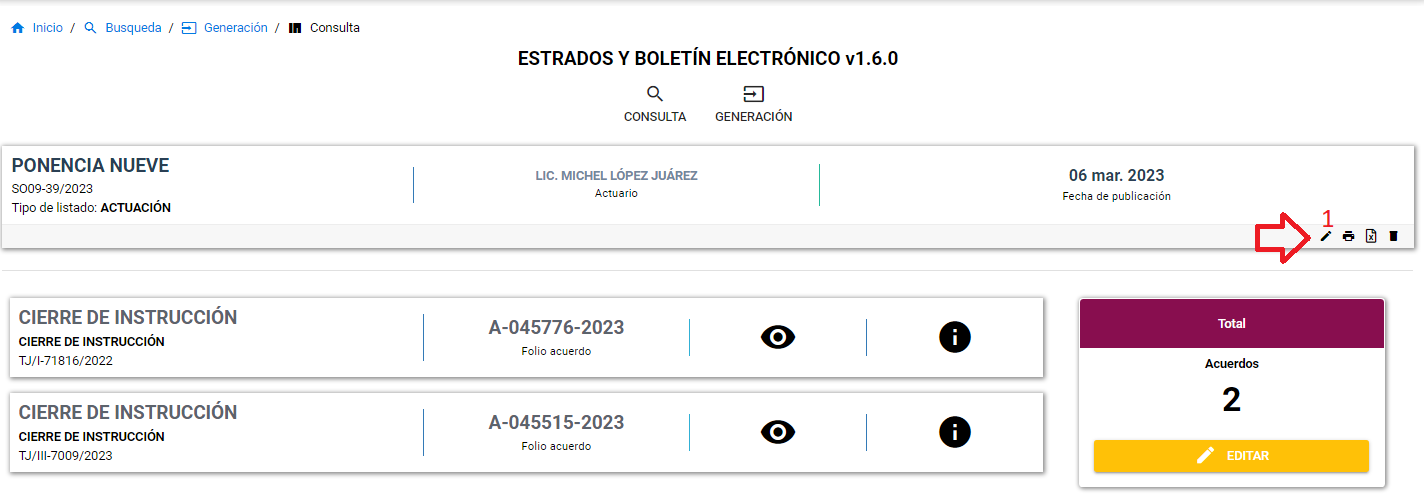
\includegraphics[width=0.88\columnwidth]{editar_acuer.png}
\end{center}

\vspace{2cm}
Se mostrará la pantalla siguiente donde podrá editar los datos deseados.

\begin{center}
    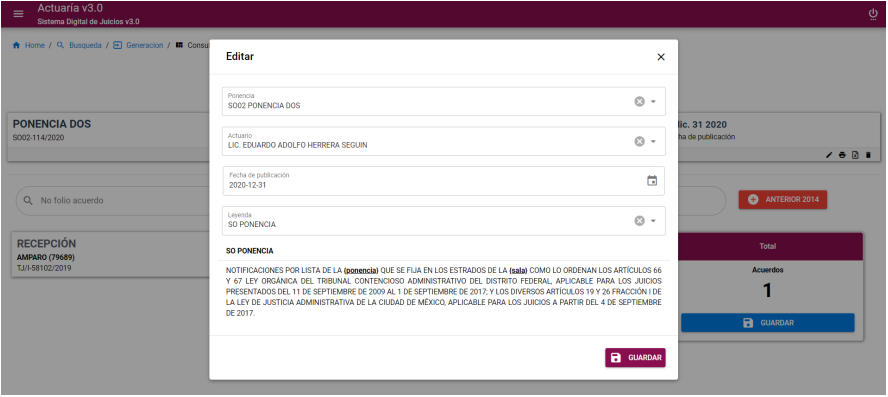
\includegraphics[width=0.88\columnwidth]{C30.png}
\end{center}

Una vez modificada la información, dar clic el botón {\bf «GUARDAR»} para que los cambios realizados se guarden correctamente. 

{\color{myblue}\section{\normalfont\sffamily{ ¿Cómo imprimir un listado?}}}\label{sec:11.1}

Hay dos maneras de imprimir un listado la primera es desde el módulo consulta dando clic en el icono {\bf {<<Imprimir>>}}

\begin{center}
    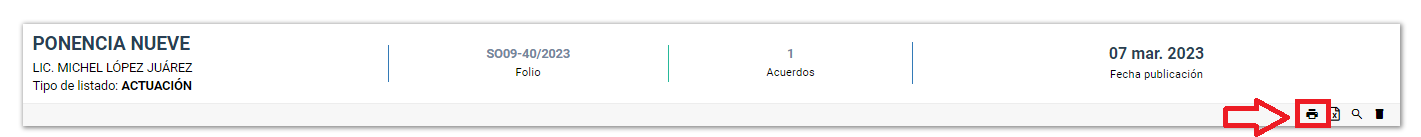
\includegraphics[width=0.88\columnwidth]{imprimir.png}
\end{center}

Se abrirá una ventana con el documento listo para imprimir

\begin{center}
    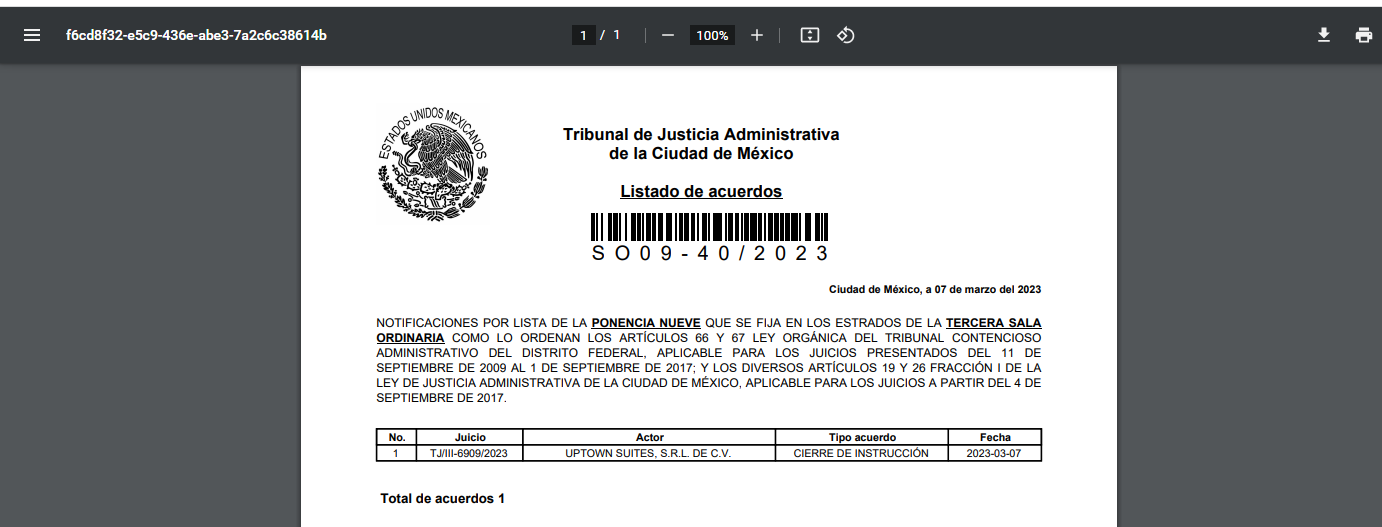
\includegraphics[width=0.66\columnwidth]{imprimir1.png}
\end{center}



\newpage
\begin{table}[t]
\begin{center}
\begin{tabular}{| c | c | c | c | }
\hline

\multicolumn{4}{ |c| }{\cellcolor[gray]{0.9}CONTROL DE VERSIONES} \\ \hline
Versión &               Elaborado por:          & Fecha de última modificación          & Motivo \\ \hline
1.0.1   & Esthefania Vidal Solares        &      12/octubre/2022
&Creación \\ \hline
1.0.2   & Esthefania Vidal Solares        &     27/febrero/2023
&Actualización \\ \hline
\hline
\end{tabular}
\caption{Control de Versiones}
\label{tab:versiones}
\end{center}
\end{table}


\end{quote}

\end{document}


t}
